\begin{figure}[ht]
  \centering
  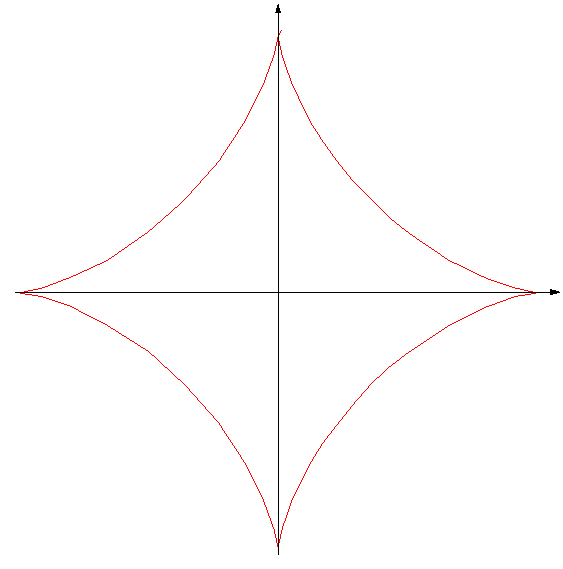
\includegraphics{Castro_2.pdf}
  \caption{Trac{\'e} de l'astro{\"\i}de}
  \label{fig:Castro_2}
\end{figure}
\begin{enumerate}
 \item 
\begin{enumerate}
 \item La courbe est sym{\'e}trique par rapport aux droites passant par l'origine et dirigées par
$\overrightarrow{i}$, $\overrightarrow{j}$, $\overrightarrow{i}+\overrightarrow{j}$.\newline
Les points $M(-t)$, $M(\pi -t)$, $M(\frac{\pi}{2}-t)$ sont respectivement les sym{\'e}triques de $M(t)$ par rapport
aux trois droites.

\item  La courbe est bir{\'e}guli{\`e}re sauf aux points o{\`u} $t$ est congru {\`a} 0 modulo $\frac{\pi }{2}$.\newline
Par raison de sym{\'e}trie, ces points sont des points de rebroussement.\newline
Au point stationnaire $M(0)$, le vecteur tangent est dirigé par la dérivée seconde
\begin{displaymath}
\overrightarrow{M^{\prime \prime }}(0) = -24a\overrightarrow{i} 
\end{displaymath}
Les tangentes aux autres points de rebroussement s'obtiennent par sym{\'e}trie. On peut noter que la tangente en
$M(\frac{\pi }{4})$ est orthogonale {\`a} la premi{\`e}re bissectrice.

\item  En notant $L$ la longueur totale de la courbe et $\overrightarrow{u}_{t}=\cos t\overrightarrow{i}+\sin t\overrightarrow{j}$, on obtient 
\begin{displaymath}
\overrightarrow{M^{\prime }}(t)=-24a\sin t\cos t~\overrightarrow{u}_{-t}=12a\sin 2t\,\overrightarrow{u}_{\pi -t} 
\end{displaymath}
d'o{\`u}
\begin{displaymath}
L = 4\int_{0}^{\frac{\pi }{2}} 
\left\Vert
\overrightarrow{M}'(t)
\right\Vert dt
= 48a\int_{0}^{\frac{\pi }{2}}\sin 2t\,dt = 48a 
\end{displaymath}
\end{enumerate}

\begin{figure}[ht]
  \centering
  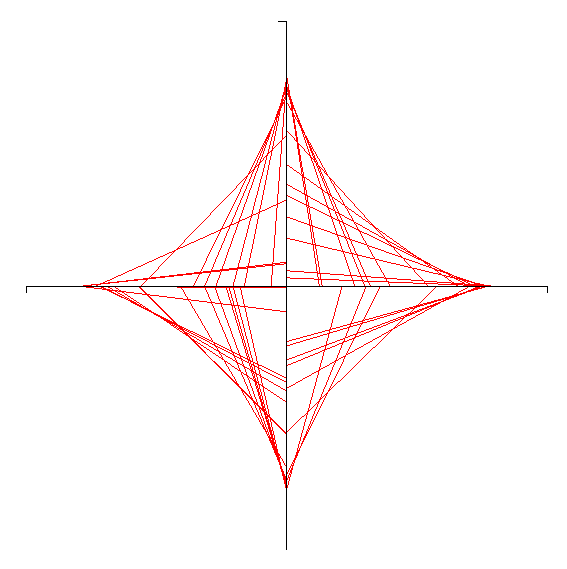
\includegraphics{Castro_1.pdf}
  \caption{Trac{\'e} de 50 segments tangents}
  \label{fig:Castro_1}
\end{figure}

\item
\begin{enumerate}
 \item Lorsque $M(t)$ n'est pas un point singulier, une {\'e}quation de $D(t)$ est
\begin{displaymath}
(x-8a\cos ^{3}t)\sin t+(y-8a\sin ^{3}t)\cos t = 0 \Leftrightarrow
x\sin t+y\cos t = 8a\sin t\cos t
\end{displaymath}


\item  On peut calculer les coordonn{\'e}es de $A(t)$ et $B(t)$. Il vient 
\begin{align*}
 \text{coordonnées de $A(t)$ : } (8a\cos t,0) & &
\text{coordonnées de $B(t)$ : } (0,8a\sin t)
\end{align*}
La longueur du segment $A(t)B(t)$ est donc constante {\'e}gale {\`a} $8a$.\newline
On peut se faire idée des tangentes à l'astroïde en faisant glisser sur les axes les deux extrémités d'un segment de longueur fixe (Fig. \ref{fig:Castro_1}). 

\begin{figure}[ht]
  \centering
  \input{Castro_3.pdf_t}
  \caption{Construction de $D(t_0)$}
  \label{fig:Castro_3}
\end{figure}
\end{enumerate}

\item
\begin{enumerate}
 \item   On cherche les $t$ tels que $D(t)$ contienne le point de coordonn{\'e}es 
\begin{displaymath}
(2a\cos t_{0},2a\sin t_{0}) 
\end{displaymath}
Ils doivent vérifier
\begin{displaymath}
4a\cos t_{0}\sin t+4a\sin t_{0}\cos t = 8a\sin t\cos t \Leftrightarrow
\sin (t+t_{0}) = \sin 2t
\end{displaymath}
La derni{\`e}re {\'e}quation {\'e}quivaut {\`a} 
\begin{align*}
 t=t_{0} &  &\text{ ou }& & t\equiv \frac{\pi -t_{0}}{3} \hspace{1cm}(\frac{\pi }{3})
\end{align*}
La deuxième relation conduit à trois tangentes faisant entre elles un angle de $\frac{\pi }{3}$.\newline
La quatrième tangente est $D(t_{0})$ qui passe par $P_{0}$ et de direction $\,\overrightarrow{u}_{\pi -t}$.

\item  D'après la question précédente, on peut construire la droite $D(t_{0})$ en remarquant qu'elle est sym{\'e}trique de $(OP_{0})$ par rapport {\`a} la droite de direction $\overrightarrow{j}$ qui passe par $P_{0}$. (Fig. \ref{fig:Castro_3})

\begin{figure}[ht]
	\centering
	\input{Castro_4.pdf_t}
	\caption{Construction géométrique de $M_0$}
\label{fig:Castro_4}
\end{figure}

\item  On note avec un indice 0 tous les objets relatifs {\`a} $t_{0}$.\newline
Cherchons $H_{0}=H(t_{0})$ sous la forme 
\begin{displaymath}
 (\lambda \sin t_{0},\lambda \cos t_{0})
\end{displaymath}
pour que $\overrightarrow{OH_0}$ soit orthogonal $D_0$. On remplace dans l'équation de $D_0$ et on obtient 
\begin{displaymath}
\lambda =8a\sin t_{0}\cos t_{0}
\end{displaymath}
puis
\begin{displaymath}
\overrightarrow{OH_{0}}+\overrightarrow{OM_{0}}=8a\,\overrightarrow{u}_{t_{0}}
\end{displaymath}
D{\'e}finissons $K_{0}$ par 
\begin{displaymath}
 \overrightarrow{OH_{0}}+\overrightarrow{OM_{0}}=\overrightarrow{OK_{0}}
\end{displaymath}
Il est sur un cercle deux fois plus grand que $\mathcal C$ et aligné avec $0$ et $P_0$. De plus,
\begin{displaymath}
 \overrightarrow{OM_{0}}=\overrightarrow{H_{0}K_{0}}
\end{displaymath}
donc $(O,M_{0},K_{0},H_{0})$ est un parall{\'e}logramme ce qui entraîne que $M_0$ est symétrique de $H_{0}$ par rapport au centre $P_{0}$ du parallélogramme.\newline
On peut donc construire $M_0$ à partir de $P_0$ (Fig. \ref{fig:Castro_4}) Sur la figure on a fait figurer $K_0$ pour éclairer la démonstration (il est utile à celle-ci mais pas à la construction).
\end{enumerate}
\end{enumerate}
%\clearpage